\documentclass[
    tikz,
    convert={outext=.svg, command=\unexpanded{pdf2svg \infile\space\outfile}},
    multi=false
]{standalone}
\usetikzlibrary{arrows, arrows.meta, automata, calc, fit, positioning, shapes}

\begin{document}
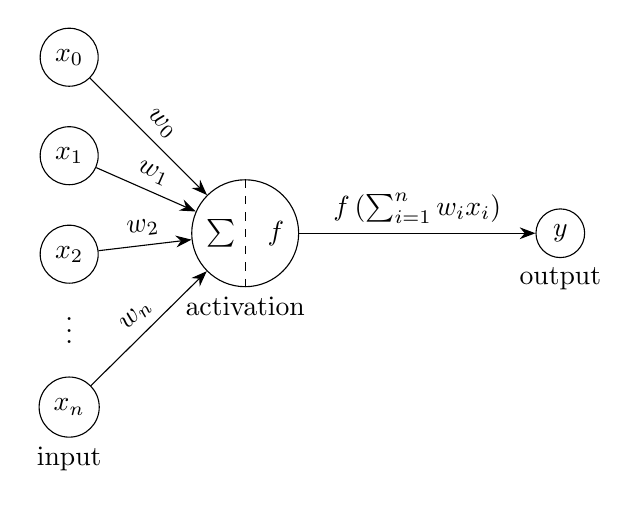
\begin{tikzpicture}[
    node distance=3cm,
    >={Stealth[length=2mm]},
    ]

    \node[draw, circle, label=below:{activation}] (unit) {$\sum\quad f$};
    \draw[dashed] (unit.north) -- (unit.south);

    \node[draw, circle, above left=2.1cm of unit] (x_0) {$x_0$};
    \node[draw, circle, below=5mm of x_0] (x_1) {$x_1$};
    \node[draw, circle, below=5mm of x_1] (x_2) {$x_2$};
    \node[below=1mm of x_2] (dots) {$\vdots$};
    \node[draw, circle, below=3mm of dots, label=below:{input}] (x_n) {$x_n$};

    \node[draw, circle, right=3cm of unit, label=below:{output}] (output) {$y$};

    \draw[->] (x_0) -- node[midway, sloped, above] {$w_0$} (unit);
    \draw[->] (x_1) -- node[midway, sloped, above] {$w_1$} (unit);
    \draw[->] (x_2) -- node[midway, sloped, above] {$w_2$} (unit);
    \draw[->] (x_n) -- node[midway, sloped, above] {$w_n$} (unit);
    \draw[->] (unit) -- node[midway, above] {$f\left(\sum_{i=1}^n w_ix_i \right)$} (output);
\end{tikzpicture}
\end{document}
